\documentclass{article}
\usepackage{mathtools}
\usepackage[nottoc]{tocbibind}
\usepackage[nohead, nomarginpar, margin=1in, foot=.25in]{geometry}
\usepackage{mathtools}
\usepackage{bbm}
\usepackage{amssymb}
\usepackage{float}  % For fixing the image in draft

\usepackage{amsmath}
\usepackage{lscape}
\usepackage{graphicx}
\graphicspath{ {./images/} }

%\usepackage{nips10submit_e}
\usepackage{graphicx,times,verbatim,amsmath,amssymb,amsthm}
%\usepackage{epstopdf}
\usepackage{natbib}
%\usepackage{mathbbold}
\usepackage{bm}
\usepackage{enumerate}
\usepackage{mathrsfs}
\usepackage{epsfig}
\usepackage{caption}
\usepackage{subcaption}
\usepackage{verbatim}
\usepackage{multirow}
\usepackage{array}

\newtheorem{theorem}{Theorem}[section]
\newtheorem{lemma}[theorem]{Lemma}
\newtheorem{corollary}[theorem]{Corollary}
\newtheorem{proposition}[theorem]{Proposition}
\newtheorem{definition}[theorem]{Definition}
\newtheorem{remark}[theorem]{Remark}
\newtheorem{condition}[theorem]{Condition}
\newtheorem{assumption}[theorem]{Assumption}
\newtheorem{property}[theorem]{Property}
\newtheorem{result}[theorem]{Result}
\newtheorem{example}[theorem]{Example}

\newtheorem*{remark*}{Remark}
\DeclareGraphicsExtensions{.eps}

\renewcommand{\baselinestretch}{1} % 2.0 or 3.0 would do.
\renewcommand*\labelenumi{(\theenumi)}
\renewcommand\theequation{\arabic{section}.\arabic{equation}}
\DeclarePairedDelimiter\ceil{\lceil}{\rceil}
\DeclarePairedDelimiter\floor{\lfloor}{\rfloor}

%\usepackage[linesnumbered,ruled,vlined]{algorithm2e}
\usepackage[linesnumbered,ruled]{algorithm2e}
\RestyleAlgo{boxruled}

\topmargin 0pt \advance \topmargin by -\headheight \advance \topmargin by
-\headsep \textheight 8.9in \oddsidemargin 0pt \evensidemargin
\oddsidemargin \marginparwidth 0.5in \textwidth 6.5in

\begin{document}
\title{Factor Analysis on Report Citations, Using a Combined Latent and logistic Model}
\author{Namjoon Suh, Xiaoming Huo, Eric Heim, Timothy Van Slyke, and Lee Seversky}

\date{\today}
\maketitle

\begin{abstract}
% To be added later...
We propose a combined latent and logistic model for the citation network, where either a latent model or a logistic model alone is often insufficient to capture the structure of the data.
    The proposed model has a latent (i.e., factor analysis) model to represents the main technological trends (aka factors), and adds a sparse logistic component that captures the remaining ad hoc dependence. Parameter estimation are carried out through construction of a joint-likelihood function of edges and properly chosen penalty terms. The convexity of the likelihood function allows us to develop an efficient algorithm, while the penalty terms generate a low-dimensional latent component and a sparse graphical structure. Simulation results are reported that show the new method works well in practical situations. The proposed method has been applied to a real application in citation network of statistician data set (Ji and Jin, 2016 \cite{ji2016coauthorship}).
\end{abstract}

\noindent{\sc KEY WORDS}: citation network, matrix decomposition, latent variable model,  logistic model, convex optimization, graphical models 

\section{Introduction}\label{sec:intro}
We study a citation network, where each node (i.e., item) can be a technical report or a publication. A node may cite another node. Associated with a pair of nodes $i$ and $j$, we denote a binary random variable $X_{ij}$, where $1 \le i,j \le n$ and $n$ is the total number of nodes. We have $X_{ij}=1$ if and only if either node $i$ cites node $j$ or vice versa; otherwise $X_{ij}=0$. For each node $i$, we assume that there is an associated binary vector $f_{i} \in \mathbb{R}^K$, such that the $k$th entry of $f_{i}$, $f_{ik} = 1$, if and only if node $i$ is related to topic (i.e., factor) $k, 1\le k \le K$. Here $K$ is the total number of underlying topics (i.e., factors, or trends). We assume a logistic model for $X_{ij}$'s: for $1\le i,j \le n$,

\begin{equation}
\label{eq:logistic01}
\mathbb{P}(X_{ij}=1) = \frac{e^{\alpha + f_i^T D f_j }}{1 + e^{\alpha + f_i^T D f_j }},
\end{equation}
here $\alpha \in \mathbb{R}$ is a parameter and matrix $D \in \mathbb{R}^{K \times K}$ is a diagonal matrix: $D = \mbox{diag}\{d_{1},d_{2},\ldots,d_{K}\}$. We assume $d_{ii} > 0$ for $1 \le i \le K$.
Another way to put \eqref{eq:logistic01} is
\begin{equation}
\label{eq:logistic02}
\mathbb{P}(X_{ij}=1) = \frac{\exp\left\{\alpha + \sum_{k=1}^K f_{ik}f_{jk}d_{k} \right\}}{1 + \exp\left\{\alpha + \sum_{k=1}^K f_{ik}f_{jk}d_{k} \right\}},
\end{equation}
A justification of the above model is that when both node $i$ and node $j$ are related to topic $k$, they have a higher chance to cite one way or the other. We have assumed a common strengthen coefficient $d_k$ ($1\le k \le K$) for factor $k$, despite different nodes. We denote a matrix $F = \{f_1, f_2, \ldots, f_n\} \in \mathbb{R}^{K \times n}$. Each column $i$ in matrix $F$ contains the factor loadings associated with the node $i$ ($1\le i \le n$). Given the diagonal matrix $D$ and the factor loading matrix $F$, we assume that $X_{ij}$'s are independent; therefore we have the total conditional probability function as follows:
\begin{equation}
\label{eq:logistic03}
\mathbb{P}(\{X_{ij}, 1\le i,j \le n\})
= \prod_{1\le i<j \le n} \mathbb{P}(X_{ij})
= \prod_{1\le i<j \le n}  \frac{e^{X_{ij}(\alpha + f_i^T D f_j) }}{1 + e^{\alpha + f_i^T D f_j }},
\end{equation}
where $\mathbb{P}(X_{ij})$ is given in \eqref{eq:logistic02}.
The last equation holds because $X_{ij}$ only takes binary (i.e., $0$ or $1$) values.
Recall that the dot product of two matrices with same dimensionality, $A,B\in \mathbb{R}^{a \times b}$, is defined as $A\bullet B=\mbox{trace}(A^T B) = \sum_{i=1}^a\sum_{j=1}^b a_{ij}b_{ij}$.
The above \eqref{eq:logistic03} can be further rewritten as
\begin{equation}
\label{eq:logistic04}
\mathbb{P}(\{X_{ij}, 1\le i,j \le n\})
= \frac{\exp(\alpha \sum_{1\le i< j\le n}X_{ij} +\frac{1}{2} X \bullet (F^T D F))}{\prod_{1\le i<j \le n}  1 + e^{f_i^T D f_j }},
\end{equation}
where we assume $X_{ii}=0$ for all $i$ ($1\le i \le n$) and $X_{ij} = X_{ji}$ for all $i$ and $j$ ($1\le i,j \le n$), i.e., the matrix $X$ is symmetric.
The above delivers a factor analysis model. Various linear and nonlinear latent variable models have been studied extensively in the literature (e.g.,\cite{joreskog1969general, mcdonald2014factor,lord2008statistical, rasch1980probabilistic, harman1960modern, joreskog1970general}).

Our work is motivated from a recent work {\it Fused Latent and Graphical (FLaG) model} (Chen et al, 2016, \cite{chen2016fused}). They assume that majority of variation of responses can be accounted by low dimensional latent vector, and remaining dependent structure of responses can be explained by sparse graphical structure. Thus, the resulting model contains a low-dimensional latent vector and a sparse conditional graph. Their key idea is to separate these two dependent structures so that they can facilitate the statistical inference. Our model also assumes that there exist two dependent structures among citation edges in network. A low-dimensional version of the aforementioned latent vector model is largely correct and majority of the citations among the nodes are induced by these common latent vectors $f_{i}$'s (with weigh coefficients $d_{i}$'s). There is still a small remainder due to the graphical component.

Though it may seem similar to Chen et al \cite{chen2016fused}, we work on a different model formulation in several aspects. First, FLaG is built to analyze the Eysenck’s Personality Questionnaire that consists of items designed to measure Psychoticism, Extraversion, and Neuroticism. So there are $p$ questions that need to be answered, and each questions fall into above three categories. If there are n respondents to questions, we have n independent data generated from same distribution. In our case, the observed citation network can be thought of as one realization of random graph. Second, FLaG set a collection of binary responses for each individual questions follow a joint distribution which is a combination of Item Response Theory (IRT) model and Ising model, whereas we model the citation edges among papers as random variables, whose dependent structure is characterized by the combination of Latent Factor Analysis model and logistic model. Last but not least, FLaG approximate the original likelihood through constructing pseudo-likelihood function by taking advantage of conditional independence among the nodes, but our model’s likelihood function is directly accessible due to the conditional independence among edges given parameters.

The proposed modeling framework is also related with the analysis of decomposing a matrix into low-rank and sparse components and the statistical inference of a multivariate Gaussian model whose precision matrix admits the form of a low-rank matrix plus a sparse matrix (\cite{chandrasekaran2010latent, candes2011robust, zhou2010stable}). However, the inference and optimization of the current model are different from those cases. We will construct a regularized-likelihood function, based on which estimator will be proposed for simultaneous model selection and parameter estimation. The optimization for the regularized estimator will be convex, for which we will develop an efficient algorithm through the alternating direction method of multiplier (ADMM : \cite{boyd2011distributed, gabay1975dual, glowinski1975solution}).

The rest of the paper is organized as follows. In section 2 we will give a presentation on how to build a model which can encode both latent dependent structure due to the common topics and remaining ad-hoc dependent structure. In section 3, we will talk about assumptions in our model and penalization on likelihood function constructed in section 2. Section 4 gives the detailed procedure on how to compute the estimator of the optimization problem in Section 3. In Section 5, we will present simple numerical experiments on synthetic data, and application of our model on real citation network of statisticians. We finally conclude this work in section 6 with several open questions remain to be solved and some directions for future research.

\section{Model Formulation}
\label{sec:model-form}

Recall the following graphical model that was established in \eqref{eq:logistic04}, which is essentially a factor model (latent variable model):
$$
\mathbb{P}(\{X_{ij}, 1\le i,j \le n\})
= \frac{\exp(\alpha \sum_{1\le i< j\le n}X_{ij} +\frac{1}{2} X \bullet (F^T D F))}{\prod_{1\le i<j \le n}  1 + e^{f_i^T D f_j }},
$$
where
$X_{ij}, 1\le i,j \le n$, are binary random variables indicating either node $i$ cites node $j$ or vice versa,
matrix $X = \{X_{ij}\} \in \mathbb{R}^{n \times n}$ is symmetric with diagonal entries all being equal to zero,
factor loading matrix $F = [f_1,f_2,\ldots,f_n]\in \mathbb{R}^{K\times n}$ records the relation between nodes and underlying topics, $F^T$ is the transpose of $F$,
and matrix $D \in \mathbb{R}^{K \times K}$  is diagonal with entries being the weight coefficients of factors.

The above specifies a latent model (or equivalently a factor model).
We now describe a graphical model in the following.
The graphical model will complement the latent model by characterizing links that are not interpretable via common factors.
For the aforementioned binary random variable $X_{ij}$, $1\le i,j \le n$, we define
\begin{equation}
\label{eq:logistic05}
\mathbb{P}(X_{ij}=1) = \frac{e^{\alpha' + S_{ij} }}{1 + e^{\alpha' + S_{ij} }},
\end{equation}
where $S_{ij} \in \mathbb{R}$, for $1\le i,j \le n$, denotes the relation between nodes $i$ and $j$.
If we have $S_{ij}=0$, then it is less likely to have a citational relationship between nodes $i$ and $j$.
On the other hand, if $S_{ij}>0$, then it is more likely to have a citation link between nodes $i$ and $j$.
Here parameter $\alpha' \in \mathbb{R}$ plays the same role as parameter $\alpha$ does in model \eqref{eq:logistic01}.
Denote the matrix $S = \{S_{ij}, 1\le i,j \le n \} \in \mathbb{R}^{n \times n}$.
Assume that given the matrix $S$, the binary random variables
$X_{ij}$'s are independent;
consequently, we have the total conditional probability function as follows:
\begin{eqnarray}
\mathbb{P}(\{X_{ij}, 1\le i,j \le n\})
&=& \prod_{1\le i<j \le n} \mathbb{P}(X_{ij}) \nonumber \\
&=& \prod_{1\le i<j \le n}  \frac{e^{X_{ij}(\alpha' + S_{ij}) }}{1 + e^{\alpha' + S_{ij} }} \nonumber \\
&=& \frac{\exp(\alpha' \sum_{1\le i< j\le n}X_{ij} +\frac{1}{2} X \bullet S)}{\prod_{1\le i<j \le n}  1 + e^{\alpha' + S_{ij} }}.
\label{eq:logistic06}
\end{eqnarray}
Recall that we have assumed that $X_{ii}=0$ for all $i$ ($1\le i \le n$) and $X_{ij} = X_{ji}$ for all $i$ and $j$ ($1\le i,j \le n$), i.e., the matrix $X$ is symmetric.
In the combined model, we integrate \eqref{eq:logistic04} and
\eqref{eq:logistic06} to render the joint conditional probability function as follows:
\begin{eqnarray}
\label{eq:logistic07}
\mathbb{P}(X \mid \alpha,  F, D, S)
&=&  \prod_{1\le i<j \le n}
\frac{e^{X_{ij}(\alpha + S_{ij} + f_i^T D f_j) }}{1 + e^{\alpha + S_{ij}+ f_i^T D f_j}} \nonumber \\
&=& \frac{\exp\left(\alpha \sum_{1\le i< j\le n}X_{ij} +\frac{1}{2} X \bullet (F^T D F) +\frac{1}{2} X \bullet S\right)}{\prod_{1\le i<j \le n}  \left(1 + e^{\alpha + f_i^T D f_j +S_{ij}}\right) }.
\end{eqnarray}

\section{Estimation}
\label{sec:estimate}


Note that in the model \eqref{eq:logistic07}, the log-likelihood function has the form as follows:
\begin{eqnarray}
\label{eq:logistic08}
\mathbb{L}(\alpha,  F, D, S; X)
&=& \alpha \sum_{1\le i< j\le n}X_{ij} +\frac{1}{2} X \bullet (F^T D F) +\frac{1}{2} X \bullet S \\
&& -\sum_{1\le i<j\le n} \log \left(1 + e^{\alpha + f_i^T D f_j +S_{ij} }\right). \nonumber
\end{eqnarray}

If we consider maximizing the above log-likelihood function,
we will encounter several technical issues which are described below.
\begin{enumerate}
\item We would like the matrix $S \in \mathbb{R}^{n \times n}$ to have as many zero entries as possible; i.e., matrix $S$ is {\it sparse.}

\item There is an identifiability issue with the formation $F^T D F$.
More specifically, let $P \in \mathbb{R}^{K \times K}$ be a signed permutation matrix, then we have $P^T P = I_n$, where $I_n \in \mathbb{R}^{K \times K}$ is the identity matrix.
Notice that matrix $F' = PF$ is also a factor loading matrix, and
matrix $D' = P D P^T$ is still a diagonal matrix;
we have
$$
F^T D F = F^T P^T P D P^T P F = (F')^T D' F',
$$
i.e., the choice of $F$ and $D$ is not unique.

\item We would like the number of nonzeros in each column of $F$ to be small, reflecting that each node is associated with a small number of underlying topics.

\item Overall, the rank of matrix $F^T D F$ cannot be larger than $\min\{n,K\}$.
With the application that we have in mind, in this paper, we assume that $K$ is much smaller than $n$.

\item To ensure unique separation of $\alpha\mathbbm{1}\mathbbm{1}^T$ and $L$, we assume that eigen-vector of $L$ is centered, that is,
\[
    JLJ = L \quad where \quad
    J=I_{n}-\frac{1}{n}\mathbbm{1}\mathbbm{1}^T
\]
This condition uniquely identifies F up to a common orthogonal transformation of its columns.

\end{enumerate}


Directly maximizing the objective function in \eqref{eq:logistic08} is not going to be an easy task.
Following the approaches that were mentioned in Introduction, we propose to relax $F^T D F$ to $L$, where $L$ is a low rank matrix.
Consequently, the log-likelihood function in \eqref{eq:logistic08} can be rewritten as
\begin{eqnarray}
\label{eq:logistic09}
\mathbb{L}_n(\alpha,  L, S; X)
&=& \alpha \sum_{1\le i< j\le n}X_{ij} +\frac{1}{2} X \bullet L +\frac{1}{2} X \bullet S \\
&& -\sum_{1\le i<j\le n} \log \left(1 + e^{\alpha + L_{ij} +S_{ij}}\right). \nonumber
\end{eqnarray}


We propose a penalize likelihood estimation approach as follows:
\begin{eqnarray}
\label{eq:logistic10}
(\hat{\alpha}, \hat{L}, \hat{S})
= \mbox{arg min}_{\alpha, L, S} \left\{
-\frac{1}{n} \mathbb{L}_n(\alpha,  L, S; X) + \gamma \|S\|_1
+ \delta \|L\|_\ast\right\},
\end{eqnarray}
where $\gamma>0$ and $\delta>0$ are algorithmic parameters whose values will be discussed later,
the $L_1$ norm of matrix $S$ is defined as $\|S\|_1 = \sum_{i\neq j} S_{ij}$ (Note that we do not penalize the diagonal entries of $S$), and nuclear norm of matrix $L$ is defined as $\|L\|_\ast = {\mbox{trace}\sqrt{(L^T L)}}$. Recall that both $S$ and $L$ are symmetric matrices. The entries of matrix $S$ can either be positive or negative. Note that we have imposed the diagonal entries of the matrix $X$ to be zeros. Given that $L = F^T D F$ where matrix $D$ is diagonal with nonnegative diagonal entries, it is easy to see that matrix $L$ is positive semidefinite; which consequently leads to $\|L\|_\ast = \mbox{trace}(L)$, which is a linear functional to the matrix $L$.
The nuclear norm of $L$ penalizes the number of nonzero eigenvalues of $L$, which is the same as the rank
of $L$.
The regularization based on the nuclear norm was proposed in \cite{fazel2001rank}
and its statistical properties are studied in \cite{bach2008consistency}.

After we have obtained $\hat{S}$ in \eqref{eq:logistic10}, we can uncover the graphical model by investigating non-zero entries in $\hat{S}$.
On the other hand when we have calculated $\hat{L}$, we may not be able to find binary matrix $F$ and nonnegative diagonal matrix $D$ such that $\hat{L} = F^T D F.$
This is the price we have to pay for an amenable computational problem. The rank of estimated $\hat{L}$ will be our estimate of the number of factors (i.e., underlying common topics). For the issue on assigning the community membership of each node $i$, we will discuss this later in Section 6.

\section{Computation}
\label{sec:compute}

We propose a method that takes advantage of the special structure
of the $L_1$ and nuclear norms by means of the
alternating direction method of multiplier (ADMM), which is a method
that has recently gained momentum.
An examination of the objective function in \eqref{eq:logistic10} unvails that
terms
\[
\alpha \sum_{1\le i< j\le n}X_{ij} +\frac{1}{2} X \bullet L +\frac{1}{2} X \bullet S
\]
are linear in $\alpha,  L$, and $S$.
The term
\[
\sum_{1\le i<j\le n} \log \left(1 + e^{\alpha + L_{ij} +S_{ij}}\right)
\]
is convex with respect to $\alpha,  L$, and $S$.
Functions $\|S\|_1$ and $\|L\|_\ast$ are known to be convex functions.
Therefore, the objective function in \eqref{eq:logistic10} is convex. The above convex optimization problem can be solved via ADMM as follows.


\subsection{ADMM approach}
\label{sec:ADMM}
We give a review of the alternating direction method
of multiplier (ADMM).
Consider two closed convex functions
$$
f : \chi_f \to \mathbb{R} \mbox{ and } g : \chi_g \to \mathbb{R},
$$
where the domain $\chi_f$ and $\chi_g$ of functions $f$ and $g$ are closed convex subsets of $\mathbb{R}^d$, and $\chi_f \bigcap \chi_g$ is nonempty.
Both $f$ and $g$ are possibly non-differentiable.
The alternating direction method
of multiplier is an iterative algorithm that solves the following generic optimization problem:
$$
\min_{x \in \chi_f \bigcap \chi_g} \left\{f(x) + g(x) \right\},
$$
or equivalently
\begin{eqnarray}
\label{eq:admm1}
\min_{x \in \chi_f, z\in \chi_g} & \left\{f(x) + g(z) \right\}, \\
\mbox{ subject to } & x = z. \nonumber
\end{eqnarray}
To describe the algorithm, we will need the following proximal operators
\begin{itemize}
\item $\mathbf{P}_{\lambda,f}: \mathbb{R}^d \to \chi_f$ as
$$
\mathbf{P}_{\lambda,f}(v) = \mbox{arg min}_{x \in \chi_f} \left\{
f(x) + \frac{1}{2\lambda} \|x-v\|^2_2
\right\}
$$

\item and $\mathbf{P}_{\lambda,g}: \mathbb{R}^d \to \chi_g$ as
$$
\mathbf{P}_{\lambda,g}(v) = \mbox{arg min}_{x \in \chi_g} \left\{
g(x) + \frac{1}{2\lambda} \|x-v\|^2_2
\right\},
$$
where $\|\cdot\|_2$ is the usual Euclidean norm on $\mathbb{R}^d$ and $\lambda$ is a scale parameter that is a fixed positive constant.
\end{itemize}
The algorithm starts with some initial values $x^0 \in \chi_f,
z^0 \in \chi_g, u^0 (=\lambda y^0) \in \mathbb{R}^d$.
At the $(m+1)$th iteration, $(x^m, z^m, u^m)$ is updated according to the following steps until convergence
\begin{itemize}
\item Step 1: $x^{m+1} = \mathbf{P}_{\lambda,f}(z^m - u^m)$,

\item Step 2: $z^{m+1} = \mathbf{P}_{\lambda,g}(x^{m+1} + u^m)$,

\item Step 3: $u^{m+1} = u^m + x^{m+1} - z^{m+1}$.

\end{itemize}
The convergence properties of the algorithm are summarized in the following result in \cite{boyd2011distributed}.
Let $p^\ast$ be the minimal value in \eqref{eq:admm1}.

\begin{theorem}[Boyd et al., 2011]
Assume functions $f: \chi_f \to \mathbb{R}$ and
$g: \chi_g \to \mathbb{R}$ are
closed convex functions, whose domains $\chi_f$ and $\chi_g$
are closed convex subsets of $\mathbb{R}^d$ and
$\chi_f \bigcap \chi_g \neq \emptyset$.
Assume the Lagrangian of \eqref{eq:admm1}
$$
L(x,z,y) = f(x) + g(z) + y^T(x-z)
$$
has a saddle point, that is, there exists $(x^\ast, z^\ast, y^\ast)$ (not necessarily unique) that $x^\ast \in \chi_f$ and
$z^\ast \in \chi_g$, for which
$$
L(x^\ast, z^\ast, y) \le L(x^\ast, z^\ast, y^\ast) \le
L(x, z, y^\ast), \qquad \forall x, z, y \in \mathbb{R}^d.
$$
Then the ADMM has the following convergence properties.
\begin{enumerate}
\item Residual convergence. $x^m - z^m \to 0$
as $m \to \infty$; i.e., the iterates approach feasibility.

\item Objective convergence. $f(x^m) + g(z^m) \to p^\ast$ as $m \to \infty$; i.e., the objective function of
the iterates approaches the optimal value.

\item Dual variable convergence. $y^m \to y^\ast$ as $m \to \infty$, where $y^\ast$ is a dual optimal point.

\end{enumerate}
\end{theorem}


Now we see how ADMM can be adopted to solve for our penalized likelihood estimation \eqref{eq:logistic10}.
We reparameterize $M = L + S$ and let $x = (\alpha, M, L, S)$ (viewed as a vector).
We define the following:
\begin{eqnarray*}
\chi_f &=& \{ (\alpha, M, L, S): \alpha\in\mathbb{R}, M, L, S \in \mathbb{R}^{n \times n},
L \mbox{ is positive semidefinite, }
S \mbox{ is symmetricg} \}, \\
f(x) &=&
-\frac{\alpha}{n} \sum_{1\le i< j\le n}X_{ij}
-\frac{1}{2n} X \bullet M %L - \frac{1}{2n} X \bullet S
+ \frac{1}{n}
\sum_{1\le i<j\le n} \log \left(1 + e^{\alpha + M_{ij}}\right)
+ \gamma \|S\|_1
+ \delta \|L\|_\ast, \\
\chi_g &=& \{ (\alpha, M, L, S): \alpha\in\mathbb{R}, M, L, S \in \mathbb{R}^{n \times n},
M \mbox{ is symmetric and } M=L+S \}, \mbox{ and }\\
g(x) &=& 0, \mbox{ for } x \in \chi_g.
\end{eqnarray*}
One can verify that \eqref{eq:logistic10} can be written as
$$
\min_{x \in \chi_f \bigcap \chi_g} \left\{f(x) + g(x) \right\}.
$$


We now present each of the three steps of the ADMM algorithm and show that the proximal
operators $\mathbf{P}_{\lambda,f}$ and $\mathbf{P}_{\lambda,g}$ are easy to evaluate.
Let
$$
x^m = (x^m_\alpha, x^m_M, x^m_L, x^m_S), \quad
z^m = (z^m_\alpha, z^m_M, z^m_L, z^m_S), \quad
u^m = (u^m_\alpha, u^m_M, u^m_L, u^m_S).
$$
Step 1. We solve $x^{m+1} = \mathbf{P}_{\lambda,f}(z^m - u^m)$.
Due to the special structure of $f(\cdot)$,
$x^{m+1}_\alpha, x^{m+1}_M, x^{m+1}_L$, and $x^{m+1}_S$
can be updated separately. More precisely, we have
\begin{eqnarray}
x^{m+1}_\alpha, x^{m+1}_M &=& \mbox{arg min}_{\alpha, M} \quad
-\frac{\alpha}{n} \sum_{1\le i< j\le n}X_{ij}
-\frac{1}{2n} X \bullet M
+ \frac{1}{n} \sum_{1\le i<j\le n} \log \left(1 + e^{\alpha + M_{ij}}\right) \nonumber \\
&& + \frac{1}{2\lambda}\left[\alpha - (z^m_\alpha - u^m_\alpha)\right]^2
+ \frac{1}{2\lambda}\|M - (z^m_M - u^m_M)\|^2_F, \label{eq:admm02} \\
x^{m+1}_L &=& \mbox{arg min}_{ L} \quad \delta \|L\|_\ast
+ \frac{1}{2\lambda}\|L - (z^m_L - u^m_L)\|^2_F,\label{eq:admm03}
\\
&& \mbox{subject to $L$ is positive semidefinite;} \nonumber \\
x^{m+1}_S &=& \mbox{arg min}_{ S} \quad  \gamma \|S\|_1
+ \frac{1}{2\lambda}\|S - (z^m_S - u^m_S)\|^2_F,
\label{eq:admm04}
\\
&& \mbox{subject to $S$ is symmetric,} \nonumber
\end{eqnarray}
where $\|\cdot\|_F$ is the matrix Frobenius norm, defined as
$\|M\|^2_F = \sum_{i,j} m^2_{ij}$ for a matrix $M = (m_{ij})$.
The problem in \eqref{eq:admm02} may not have a closed-form solution. We use a simple gradient descent to solve this step, setting the step size, $\alpha=0.1$ and stopping criteria, $\max(|x_{\alpha,m}^{(t+1)}-x_{\alpha,m}^{(t)}|,\|x_{M,m}^{(t+1)}-x_{M,m}^{(t)}\|_{\infty}) \leq 10^{-9}$. Note that there are close-form solutions to \eqref{eq:admm03} and \eqref{eq:admm04}, while \eqref{eq:admm02} is a unconstrained convex optimization problem. More specifically, in \eqref{eq:admm03}, suppose the eigenvalue decomposition of the symmetric matrix $(z^m_L - u^m_L)$ can be written as
$$
z^m_L - u^m_L = T \Lambda T^T,
$$
where $T$ is orthogonal ($T T^T = I_n$), then, for $J=I_{n}-\frac{1}{n}\mathbbm{1}\mathbbm{1}^T$, we have
$$
x^{m+1}_L = J (T \mbox{diag}(\Lambda-\lambda \delta)_+ T^T)J^{T},
$$
and diag$(\Lambda-\lambda \delta)_+$ is a diagonal matrix with the $j$th
diagonal entry being
$$
(\Lambda_{jj}-\lambda \delta)_+ = \left\{
\begin{array}{ll}
0, & \mbox{ if } \Lambda_{jj} < \lambda \delta \\
\Lambda_{jj}-\lambda \delta, & \mbox{ if } \Lambda_{jj} \ge \lambda \delta .
\end{array}
\right.
$$
In \eqref{eq:admm04}, we have, for $i \neq j$,
\[
S_{ij} = \left\{
\begin{array}{ll}
0, & \mbox{ if } |(z^m_S - u^m_S)_{ij}| < \lambda \gamma  \\
(z^m_S - u^m_S)_{ij}-\lambda\gamma , &
\mbox{ if } (z^m_S - u^m_S)_{ij} > \lambda \gamma \\
(z^m_S - u^m_S)_{ij}+\lambda\gamma , &
\mbox{ if } (z^m_S - u^m_S)_{ij} <- \lambda \gamma
\end{array}
\right.
\]
\\

\noindent
Step 2. We solve $z^{m+1} = \mathbf{P}_{\lambda,g}(x^{m+1} + u^m)$.
A close-form solution exists here.
Denote
$
\bar{\alpha} = x^{m+1}_\alpha + u^m_\alpha,
\bar{M} = x^{m+1}_M + u^m_M,
\bar{L} = x^{m+1}_L + u^m_L$, and
$\bar{S} = x^{m+1}_S + u^m_S,
$
then evaluating $\mathbf{P}_{\lambda,g}(x^{m+1} + u^m)$ becomes
\begin{eqnarray*}
\min_{\alpha,M,L,S} & \quad
\frac{1}{2}[\alpha - \bar{\alpha}]^2
+ \frac{1}{2}\|M - \bar{M}\|^2_F
+ \frac{1}{2}\|L - \bar{L}\|^2_F
+ \frac{1}{2}\|S - \bar{S}\|^2_F  \\
\mbox{ subject to } & M \mbox{ is symmetric and } M=L+S.
\end{eqnarray*}
The above optimization problem has a close-form solution, which is as follows:
\begin{eqnarray*}
z^{m+1}_\alpha &=& \bar{\alpha}, \\
z^{m+1}_M &=&
\frac{1}{3} \bar{M} + \frac{1}{3} \bar{M}^T + \frac{1}{3} \bar{L} + \frac{1}{3} \bar{S} \\
z^{m+1}_L &=&
\frac{1}{6} \bar{M} + \frac{1}{6} \bar{M}^T + \frac{2}{3} \bar{L} - \frac{1}{3} \bar{S} \\
z^{m+1}_S &=&
\frac{1}{6} \bar{M} + \frac{1}{6} \bar{M}^T - \frac{1}{3} \bar{L} + \frac{2}{3} \bar{S}.
\end{eqnarray*}

\noindent
Step 3. We solve $u^{m+1} = u^m + x^{m+1} - z^{m+1}$, which is a simple arithmetic. \\

The most important implementation details of this algorithm are the choice of $\lambda$ and stopping criterion. In this work, we simply choose $\lambda = 0.5$. We terminate the algorithm  when in $mth$ iteration, $\|x^{m}_M - x^{m}_L - x^{m}_S\|_F \leq \delta$, with $\delta=10^{-7}$.

\section{ Numerical analysis and Applications}
In this section, we have conducted a small empirical study of measuring the performance of our proposed method with artificially specified graphical structures. Also we perform a real data analysis with citation network for statisticians.

\subsection{Synthetic data}
\textbf{Data Generation} Following the notation of our paper, each edge $X_{ij}$ follows Bernoulli distribution, whose parameter is parameterized by the probability, $P_{ij}=\frac{\exp (
\alpha+F_{i}^{T}DF_{j} +  S_{ij})}{1+\exp(\alpha+F_{i}^{T}DF_{j}+S_{ij})}$. For sparse component $S$, we generate random numbers uniformly distributed over the indices of upper triangular part (off diagonal) of matrix $S$, and make it symmetry. $F^{T}$ binary matrix has $\floor{\frac{n}{K}}$ ones in each columns, and has exactly one 1 in each rows.
We randomly choose one of rows, fill that row with ones, and project the column space of $F$ onto the orthogonal complement subspace of $\mathbbm{1}$ vector by multiplying $I_{n}-\frac{1}{n}\mathbbm{1}\mathbbm{1}^T$ to $F$. Diagonal elements of $D$ are generated from $unif[7,8]$, and alpha is generated from $unif[-3,-2]$. We set $K=3,4,5$, $n=30,80,120$, and $nnz = 10, 20, 40$, where $nnz$ denotes number of non-zero component of upper-triangular part of S.\\

\noindent \textbf{Choosing tuning parameter}
We have to admit the fact that choosing good tuning parameter is an important but challenging issue in our problem.
In our problem where the observation can be seen as one realization of random graph, it is confusing whether to define the total number of observations as $N=\frac{n(n-1)}{2}$ or 1, since in usual BIC definition, we define effective sample size "n", when we have n i.i.d. observations. Our experience shows that both BIC and AIC tend to choose the model with smallest K and no ad-hoc dependency. As an alternative, we choose a purely heuristic approach. Following the Ji and Jin \cite{ji2016coauthorship}, we plot the largest 20 eigenvalues of adjacency matrix X, which can tell us the numbers of communities embedded in network. Then, we record the rank of L and number of non-zero elements in S for each tuning parameter pair on grid, and choose proper pair of tuning parameters which can give us interesting interpretation of data. \\

\begin{figure}[h]
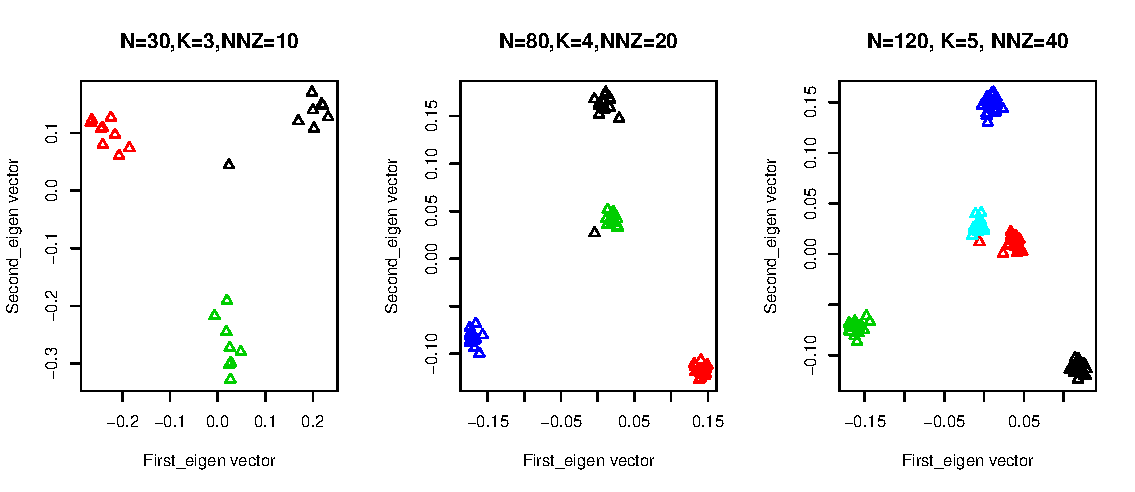
\includegraphics[width=1\textwidth]{Fig1.pdf}
\caption{\it After fitting the model, result of application of $k$-means algorithm on first $K$ eigenvectors of $\hat{L}$ matrix. (Different color represents different clusters of nodes $k$-means assign for three synthetic settings.) }
\label{fig:figure1}
\end{figure}

\noindent \textbf{Community memberships of each nodes} Given a network data, after fitting the model with a proper pair of tuning parameters, $(\gamma,\delta)$, we need to determine whether node $i$ belongs to topic $k$. We applied a simple $k$-means clustering on the fitted $L$ matrix's first $K$ eigenvectors. Furthermore, we find one interesting phenomenon. Coordinates of each rows from first two eigenvectors of estimated $\hat{L}$ matrix in our model characterize the clustering behavior of embedded topics reasonably well. Our experience shows that with only first two eigenvectors of $\hat{L}$, we can also cluster the nodes comparably well. \\

\noindent \textbf{Ad-hoc links} Ad-hoc links of synthetic network data can be thought of as $"$across edges$"$ between clusters of nodes. Since indices of non-zero entries of $S$ are randomly chosen, there might be some indices of non-zero $S_{ij}$ entries where $L_{ij}$ is also non-zero. In this case, this makes the edges indistinguishable if they come from $S_{ij}$ or $L_{ij}$. Some of "across

\noindent edges" are also attributed to $\alpha$, and unfortunately, our algorithm cannot make a difference whether the edge comes from $\alpha$ or $S_{ij}$. So the total number of across edges might not be exactly same as we set in our data generation setting. \\

\noindent \textbf{Simulation Results} Our goal in this simulation experiment is to check if our model can cluster each nodes into correct communities. Also to see if it can separate the ad-hoc links from edges which come from common topics. Tuning parameter pairs, $(\gamma,\delta) = (0.01,0.03),(0.004,0.014),(0.003,0.013)$ respectively, give us the desirable results for 3 cases. Note that different dynamics of network requires different choices of tuning parameters even the synthetic setting is same, since we are generating the random graph. However, we set the seeds in our simulation so that the results are reproducible. $Fig1$ shows us the result of clustered nodes using $k$-means algorithm on first $K(=rank(\hat{L}))$ eigenvectors. We plot the rows of first two eigenvectors on plane since it tends to visualize well the clustering behavior of nodes. Our model chooses well the ad-hoc links between clusters of nodes as can be verified in $Fig2$. We color the edges in blue whose corresponding elements of estimated $\hat{S}$ are non-zero, and black whose corresponding entries of $\hat{S}$ are zero.

\begin{figure}[b]
\begin{center}
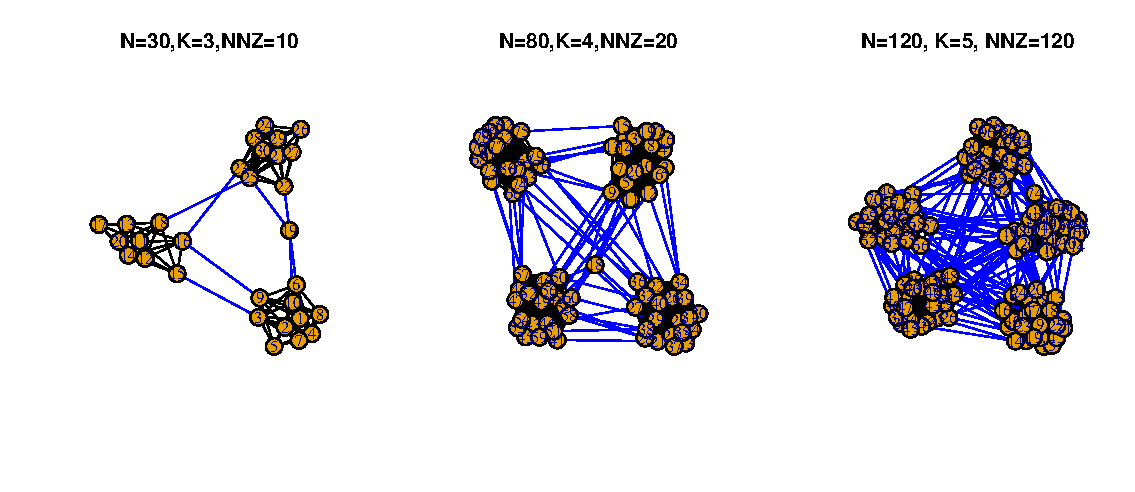
\includegraphics[scale=0.75]{Fig2.pdf}
\caption{\it Edges colored with blue correspond to non-zero entries of estimated $\hat{S}$ matrix. For all three cases, our algorithm correctly separates the "across edges" from edges coming from low-rank matrix structure.}
\end{center}
\label{fig:figure2}
\end{figure}

\subsection{Citation and Co-authorship networks for statisticians }
Recently, Ji and Jin \cite{ji2016coauthorship} published an interesting data set on citation  and co-authorship networks of statisticians. Citation relationship over 3000 papers from 4 statistical journals, published between 2003 and 2012, were collected, and collaborative network between authors of papers is given as well. In this section, we analyze the citation network. \\

\noindent\textbf{Citation Network} This dataset is based on all published papers from 2003 to first half of 2012, in 4 of the top statistical journals: Annals of Statistics, Biometrika, Journal of American Statistical Association and Journal of Royal Statistical Society (Series B). Among  3248 papers, we restrict our attention on papers which have greater than or equal to 7 citations from collected papers in original dataset. We have 543 papers in our hands. The elbow points of the scree plot may be at the 3rd, 7th, or 9th largest eigenvalue, suggesting that there might be from 2 to 8 topics in network. In light of this, we performed our analysis under the assumption that there might exist 2 distinct topics and one giant component in which 3 or 4 topics mixed up. \\

\noindent $(\gamma,\delta) = (0.000912,0.0097)$ gives us $\hat{L}$ with rank 3, and $\hat{S}$ with $|supp(\hat{S})|=197$. We apply $k$-means algorithm on 3 eigenvectors of estimated $\hat{L}$ matrix, and visualize the result of clustering by plotting the rows of first two eigenvectors of $\hat{L}$ on plane in $Fig 4$. 404 papers colored in green are densely clustered nearby the origin with a short tail, $(Fig 4)$, and $k$-means classifies these papers as third topic. We list the first two topics discovered through our analysis. (Full lists of papers for each communities are provided in $\it https://sites.google.com/site/namjoonsuh/publications$)

\begin{itemize}
  \item "Variable selection (85 papers)"
  \item "Multiple Hypothesis Testing (54 papers)"
\end{itemize}

\noindent These two topics are classical research topics in field of statistics. First group talks about "Variable selection" in high-dimensional data. Majority of papers in second community study about "Controlling False Discovery Rate" in various statistical settings. As expected, third group is quite hard to interpret and seems to have substructures. For further investigation on this group, after obtaining the sub-network which is comprised only with papers in third group, we performed same analysis once again under the assumption that $K=4$. We obtain four sub-communities as follows:

\begin{itemize}
  \item "Non-parametric Bayesian Statistics (17 papers)"
  \item "Functional Data analysis (35 papers)"
  \item "Dimension Reduction (23 papers)"
  \item "Mixed topics (329 papers)"
\end{itemize}

\begin{figure}[b]
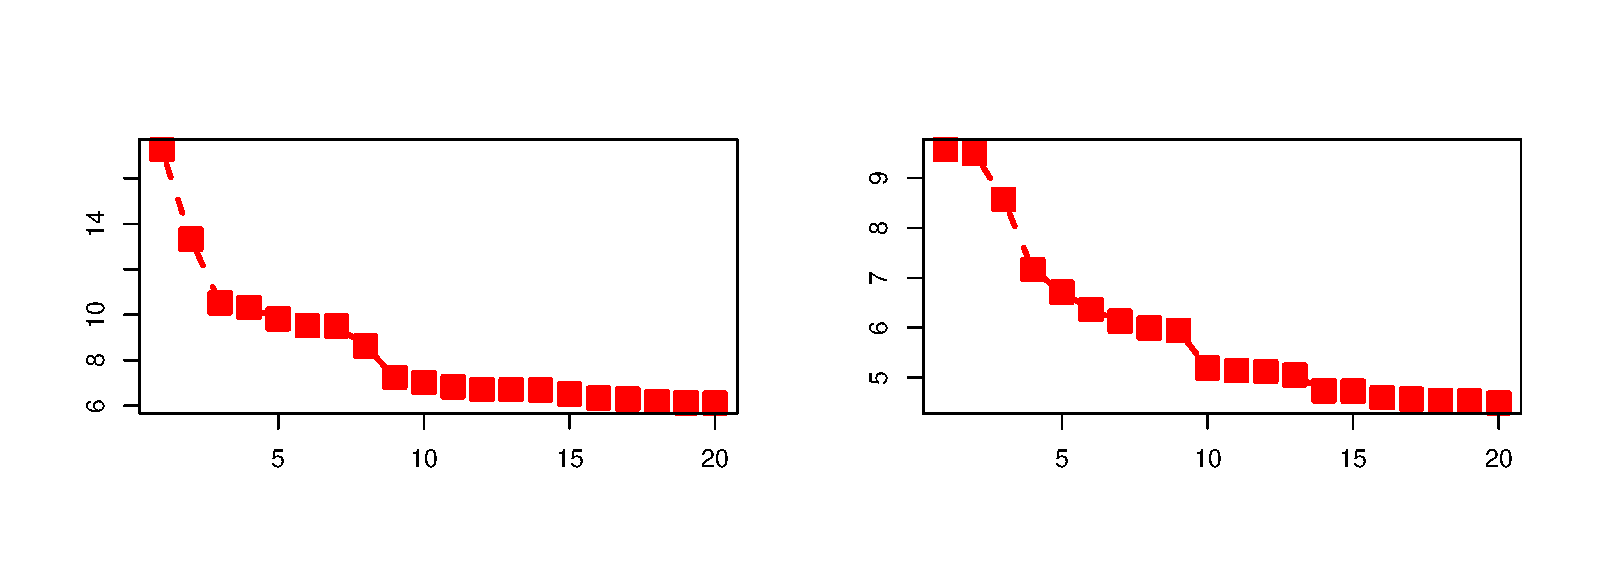
\includegraphics[width=1\textwidth]{Fig4.eps}
\caption{\it Scree plots. From left to right: 543-Citation network, Mixed Topics-Citation network.}
\label{fig:figure4}
\end{figure}

\noindent Out of this one big chunk, we got three small, but meaningful topics: "Bayesian Statistics", "Functional/longitudinal data analysis", "Dimension Reduction". Due to small volume of each communities, we could check that false discoveries for each community are all zero.\\

\noindent Sub-network structure has also a big chunk of papers which we refer to as "Mixed Topics". Not only could we see the papers with topics on "Learning Theory", "Non-parametric/semi-parametric statistics", "Spatial Statistics", "Theoretical Machine Learning", which does not seem to belong to any of five communities listed above, but also we could identify the papers with combinations of two or three topics. Papers like "The Bayesian Lasso (T Park, et al. 2008)", "Coordinate-independent sparse sufficient dimension reduction and variable selection (X Chen, et al. 2010)" are the examples of these papers. It is also interesting to think about a reason on papers which seem to have obvious membership in one of 5 communities other than Mixed topic classified as Mixed topic. For instance, "On the "degrees of freedom" on the LASSO (H Zou, et al. 2007)" is classified as Mixed Topic paper. We can simply guess model selection has lots of applications in other topics, so it might cite or have been cited by many papers in other communities. Actually, out of 19 citation relationships it has with other papers, 12 of them came from the relationships with papers from Mixed topics. \\

\noindent It is worth to note that our result is consistent with that from Ji and Jin in a sense that they also recover "Multiple Testing", "Variable selection" and "non-parametric Bayesian statistics". This is interesting since even though the dataset we consider is different from theirs, result is consistent. They focus their attentions on analyzing {\it "weakly connected giant component"} for a citation network of each paper's authors ({\it i.e. each node is an author}). We consider the citation network of papers whose node degree is greater than or equal to 7.\\

\noindent\textbf{Ad-hoc links} Non-zero components of $\hat{S}$ capture the citation relationships among papers that are not attributable to the common topics. The model we select has 197 sparse edges (9\% of total edges), and all of them are positive edges. In Table 1, we provide 15 pairs of papers that have the most positive edges. All the 15 edges come from pairs of papers from different communities. For instance, the first pair of papers comes from Functional Analysis $(\it FuncAn)$ community and Variable selection $(\it VarSel)$ community. $\it FuncAn$ paper cites $\it VarSel$ paper for borrowing a mathematical representation to build a theorem. Though it might seem to be a crucial step for building a theorem in their paper, we cannot say that two papers are closely related in terms of topic. Second pair comes from $\it MulT$  and $\it VarSel$ community. $\it MulT$ paper briefly mention about $\it VarSel$ paper in future work section, suggesting a possible way of combining their work and work in $\it VarSel$ paper.  And we also observe that as the weight of edges decreases, increasing number of pairs of papers both come from "Mixed topics" community. \\

\begin{figure}[!t]
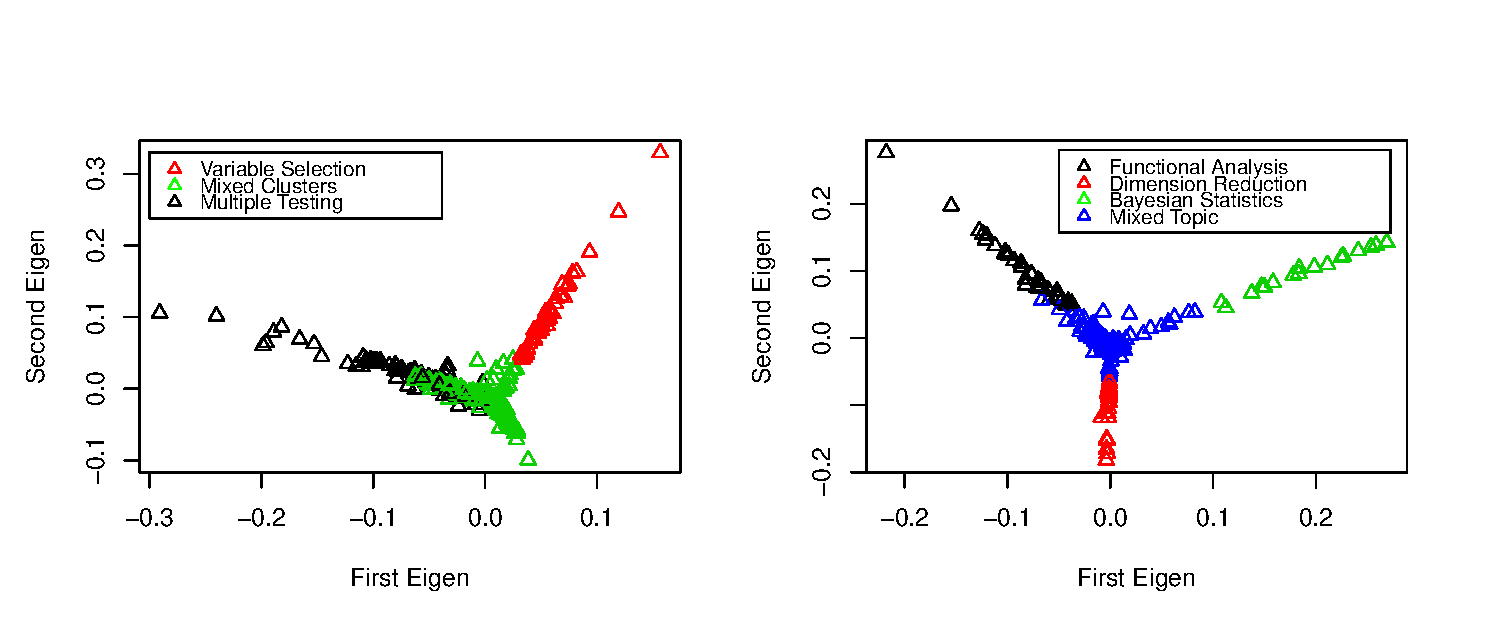
\includegraphics[width=1\textwidth]{Fig3.eps}
\caption{Illustration of first two eigenvectors of estimated $\hat{L}$ matrix for original
citation network with 543 papers(left) and sub-network graph(right). Presentation
on clustering results of k-means algorithm with different colors.}
\label{fig:figure1}
\end{figure}


\section{Conclusion}
We propose a new combined latent factor analysis and logistic model. We consider the regularized likelihood by means of $\ell 1$ and nuclear norm penalties. The computation of the regularized estimator is facilitated by developing an algorithm based on the alternating direction method of multiplier to optimize a non-smooth and convex objective function. The proposed method is applied to citation and co-authorship network of statisticians, and the estimated model renders good interpretative power. Specifically, our analysis on statistician's citation network sheds the new light on the interpretation of dataset.

However, there are still several open problems which require us to do more careful analysis. First of all, it remains unclear on how to choose the proper tuning parameters. Classical methods for choosing tuning parameters such as BIC or AIC did not work in our case, since they tend to choose the most parsimonious models. We also do not have systematic ways to do cross validation in network data. Not only because it is computationally expensive procedure, but also because if we partition the network data, we can loose fair amount of information on dependent structures among edges. This problem is also closely related with determining the number of communities in network. In lieu of using BIC or AIC, our analysis is heavily relying on heuristic approach when choosing the tuning parameter, and during this procedure, we use the screeplot for determining number of communities in network. Screeplot approach works usually well, but it does not necessarily always guarantee the correct estimate of number of communities. We need a more reliable and theoretically well understood way to determine $K$.

Secondly, we only consider the undirected case which is somewhat unrealistic assumption in real citation network, in a sense that it is not usual for two papers to cite each other at the same time. Since in our research, we were interested in separating the low rank structure of edges and ad-hoc links in network, we did not take into account the directionalities of edges in our model. However, it would be interesting to think about the way to incorporate the directed network into our matrix decomposition framework.

Last but not least, when we assign the memberships of each nodes, we use $k$-means clustering algorithm. However, $k$-means algorithm turns out that it tends to assign nodes conservatively to each communities. For example, in $Fig 4 (a)$, we can see that bunch of Multiple Testing papers are assigned as Mixed cluster, and in $Fig 4 (b)$ also, many papers which should have been classified to among three communities other than mixed topic, have been assigned as Mixed topic community. This is probably because $k$-means does not allow overlapping membership of each nodes. It would be interesting to see what happens if we apply some clustering methods which allow the overlapped memberships of nodes in network.

\section{ On non-asymptotic error bound of the estimator }
Chen et al.\cite{chen2016fused} show that their estimator recovers the algebraic structure, that is, the conditional graph structure and the number of latent variables, with probability tending to one. However, their analysis only allows a growing number of sample points whereas they keep the number of variables fixed. Their result thus severs from the tradition to analyze the more challenging high-dimensional setting, where the number of variables is also explicitly tracked. Our analysis will focus on getting a non-asymptotic error bound of estimator in the context of where the sample size is fixed as 1, and the number of nodes is growing. Readers can find more detailed descriptions on the differences between Chen et al. \cite{chen2016fused} and our model in terms of model formulation in Introduction section. We are interested in solving following optimization problem :

\begin{equation}\label{eq:1}
\min\limits_{\alpha \in R, S = S^T \atop L \succ 0}
-\frac{1}{n} \log \prod_{1\le i,j\le n}\frac{exp\left(X_{ij}\left(\alpha+
L_{ij}+S_{ij}\right)\right)}{1+exp\left(\alpha+
L_{ij}+S_{ij}\right)} + \delta \|L\|_\ast + \gamma \|S\|_1
\end{equation}

Astute readers might notice the slight difference of first term in objective function between (\ref{eq:logistic10})
and (\ref{eq:1}). (\ref{eq:1}) sums over the all $(i,j)$ pairs. Due to the symmetry of $X$ and $\Theta=\alpha\mathbbm{1}\mathbbm{1}^T+L+S$, after scaling, the only difference lies in the inclusion of diagonal term of $\Theta$.
It should be noted that this slight modification neither leads to theoretical consequences nor noticeable difference in practice.
Rather, this formulation allows us to simplify the theoretical investigation in a direction to which we want to pursue \cite{ma2017exploration}. Let ($\hat{\alpha},\hat{L},\hat{S}$) be the solution to (\ref{eq:1}), and ($\alpha^{*},L^{*},S^{*}$) be the ground truth which governs the data generating process. Let $\hat{\Theta},\Theta^{*}$ be defined respectively as, $\hat{\Theta} = \hat{\alpha}\mathbbm{1}\mathbbm{1}^T+\hat{L}+\hat{S}$ and $\Theta^{*} = \alpha^{*}\mathbbm{1}\mathbbm{1}^T+L^{*}+S^{*}$.
And denote the error term for each parameter as $\hat{\Delta}^{\Theta} = \hat{\Theta}-\Theta^{*},
\hat{\Delta}^{\alpha} = \hat{\alpha}-\alpha^{*},
\hat{\Delta}^L = \hat{L}-L^{*},
\hat{\Delta}^S = \hat{S}-S^{*}.$
Throughout the discussion, let $P^{*}=\big\{\frac{\exp(\Theta_{ij}^{*})}{1+\exp(\Theta_{ij}^{*})}\big\}_{1 \leq i,j \leq n} \in \mathbb{R}^{n \times n}$. We impose following assumptions for theoretical guarantees.

\begin{assumption} (\textbf{Strong convexity})
For any $\Theta \in \mathbb{R}^{n\times n}$, define the log-likelihood in (\ref{eq:1}), $h(\Theta) = -\frac{1}{n}\sum_{i,j} \big\{ X_{ij}\Theta_{ij} - \log(1+\exp(\Theta_{ij})) \big\}$.We assume that $h(\Theta)$ is $\tau$-strongly convex in a sense that lowest eigenvalue of Hessian matrix of likelihood function is bounded away from zero ($\tau > 0$):
\[
\nabla^{2}h(\Theta) = diag\Big(vec\Big(\frac{\exp(\Theta)}{n(1+\exp(\Theta))^{2}}
\Big)\Big) \succcurlyeq \tau I_{n^{2} \times n^{2}}
\]
For any vector $a$, diag(a) is the diagonal matrix with elements of a on its diagonal. For any square matrix A and B, $ A \succcurlyeq B $ if and only if A-B is positive semi-definite.
\end{assumption}

\begin{assumption} (\textbf{Identifiability of $\alpha\mathbbm{1}\mathbbm{1}^T$ and L, Spikiness of L})
To ensure the identifiability of $\alpha\mathbbm{1}\mathbbm{1}^T$ and L, we assume the latent variables are centered, that is $JL=L$, where $J=I_{n}-\frac{1}{n}\mathbbm{1}\mathbbm{1}^T$, $\mathbbm{1}$ denotes all one vector in $\mathbb{R}^{n}$. We impose a spikiness condition $\|L\|_{\infty}\leq\frac{\kappa}{\sqrt{n \times n}}$ on L, to ensure the separation of L and S matrix \cite{agarwal2012noisy}. We would also note that the constraint $|\alpha|\leq C\kappa$, for an absolute constant $C$, is included partially for obtaining theoretical guarantees.
\end{assumption}

With these assumptions we present the behavior of non-asymptotic error bound of our estimator through following theorem. In our result, we measure error using the squared Frobenius norm summed across both matrices:
\[
    e^{2}(\hat{\alpha}.\hat{L},\hat{S}):=\|\alpha^{*}-\hat{\alpha}\|_{F}^{2} + \|L^{*}-\hat{L}\|_{F}^{2} + \|S^{*}-\hat{S}\|_{F}^{2}
\]

\begin{theorem}
Under the assumptions (4.1) and (4.2),
if we solve the convex problem (\ref{eq:1}) with a pair of regularization parameter $(\delta,\gamma)$ satisfying
\begin{align}
\delta \geq 4\|\frac{1}{n}(X-P^{*})\|_{op} \quad and \quad \gamma \geq 4\|\frac{1}{n}(X-P^{*})\|_{\infty}+4\kappa\tau\bigg(\frac{Cn+1}{n} \bigg)
\end{align}
There exist universal constants $c_{j}$, j = 1,2,3,  for all integers $k = 1,2,...,n$ and $s = 1,2,...,n^{2}$, where $k = rank(L^{*}), s= |supp(S^{*})|$, we have following upper bound on $e^{2}(\hat{\alpha}.\hat{L},\hat{S})$
\begin{align}
    e^{2}(\hat{\alpha},\hat{L},\hat{S}) \leq
    c_{1}\frac{\delta^{2}}{\tau^{2}} +
    c_{2}\frac{\delta^{2}}{\tau^{2}}
    \bigg\{k + \frac{\tau}{\delta}\sum_{j=k+1}^{n}\sigma_{j}(L^{*})\bigg\} +
    c_{3}\frac{\gamma^{2}}{\tau^{2}}
    \bigg\{s + \frac{\tau}{\gamma}\|S^*_{M^\perp}\|_{1}\bigg\}
\end{align}
\end{theorem}

\begin{proof}
Through the assumption of strong convexity on $h(\Theta)$, and by the Taylor expansion, we can get a following lower bound on term $h(\hat{\Theta})-h(\Theta^{*})$ :

\[
h(\hat{\Theta})-h(\Theta^{*}) \geq
\langle\, \nabla_{\Theta}h(\Theta^{*}),\hat{\Theta}-\Theta^{*}\rangle\
+ \frac{\tau}{2}\|\Delta_{\hat{\Theta}}\|_{F}^{2}
\]

Hence, we can rearrange the term in (\ref{eq:2}) as follows:

\begin{equation}\label{eq:3}
    \frac{\tau}{2}\|\hat{\Delta}^{\Theta}\|_{F}^{2} \leq
    -\langle\,\nabla_{\Theta}h(\Theta^{*}),\hat{\Theta}-\Theta^{*}\rangle\
    + \delta \|L^{*}\|_\ast + \gamma \|S^{*}\|_1
    - \delta \|\hat{L}\|_\ast - \gamma \|\hat{S}\|_1
\end{equation}

Here, we introduce another notation, for any pair of positive tuning parameters $(\delta,\gamma)$ which is defined as the weighted combination of the two regularizers :
\[
\mathbb{Q}(L,S)   := \|L\|_{*} + \frac{\gamma}{\delta}\|S\|_1
\]
Through the definition of $\mathbb{Q}$, we can rewrite (\ref{eq:3}) as follows:
\begin{equation}\label{eq:4}
    \frac{\tau}{2}\|\hat{\Delta}^{\Theta}\|_{F}^{2} \leq
    -\langle\,\nabla_{\Theta}h(\Theta^{*}),\hat{\Theta}-\Theta^{*}\rangle\
    + \delta \mathbb{Q}(L^{*},S^{*}) - \delta \mathbb{Q}(\hat{\Delta}^L + L^{*},\hat{\Delta}^S + S^{*})
\end{equation}

According to Agarwal et al \cite{agarwal2012noisy}'s second element of lemma 1,
the difference $\mathbb{Q}(L^*,S^*)- \mathbb{Q}(\hat{\Delta}^L + L^{*},\hat{\Delta}^S + S^{*})$ is upper-bounded by

\begin{equation}\label{eq:5}
    \mathbb{Q}(\hat{\Delta}^L_{A},\hat{\Delta}^S_{M}) - \mathbb{Q}(\hat{\Delta}^L_{B},\hat{\Delta}^S_{M^\perp})
    +2 \sum_{j=k+1}^{n} \sigma_{j}(L^*) + 2\frac{\gamma}{\delta}\|S^*_{M^\perp}\|_{1}
\end{equation}

Here we define $S^{*}$ to be decomposable with respect to the pair of subspace $(\mathbb{M},\mathbb{M}^{\perp})$, and let $L^{*}$ be decomposable with respect to the pair of subspace $(\mathbb{A},\mathbb{B})$.

The decomposability of elementwise $\ell 1$ norm and nuclear norm with respect to a properly chosen pair of subspace is studied at length in the paper [1]. We briefly mention the concept of decomposability here for clarification:

For arbitrary subset $S \subseteq \{1,2,..,n\} \times \{1,2,..,n\}$ of matrices indices, consider the subspace pair
\[
    \mathbb{M}(S) := \{U\in R^{n \times n} | U_{ij} = 0, \forall (i,j) \not\in S \}
\]
and $\mathbb{M}^\perp(S)$. It is easy to verify that any pair of matrices $U\in \mathbb{M}(S)$ and $U' \in \mathbb{M}^\perp(S)$ in elementwise $\ell 1$ norm is decomposable in a sense that $\|U+U'\|_1 = \|U\|_1 + \|U'\|_1$. Similarly, in nuclear norm, if we define a pair of subspace $(\mathbb{A},\mathbb{B})$ for any matrix $L \in R^{n \times n}$, whose eigen decomposition is $UDV^{T}$, as follows:
\begin{align*}
    \mathbb{A}(L) := \{\Theta \in R^{n \times n} | row(\Theta) \subseteq V, col(\Theta) \subseteq U \} \\
    \mathbb{B}(L) := \{\Theta \in R^{n \times n} | row(\Theta) \subseteq V^{\perp}, col(\Theta) \subseteq U^{\perp} \}
\end{align*}
For any pair of matrices, $U\in \mathbb{A}(L)$ and $U' \in \mathbb{B}(L)$, it is also easy to check that $\|U+U'\|_\ast = \|U\|_\ast+\|U'\|_\ast$.

First, we want to control upper bound of the term $-\langle\,\nabla_{\Theta}h(\Theta^{*}),\hat{\Theta}-\Theta^{*} \rangle\$$
in (\ref{eq:4}).
\begin{align}
-\langle\,\nabla_{\Theta}h(\Theta^{*}),\hat{\Theta}-\Theta^{*} \rangle\
&=\langle\, \frac{1}{2n} (X - P), \hat\Delta^{\alpha\mathbbm{1}\mathbbm{1}^T} + \hat\Delta^{L} + \hat\Delta^{S} \rangle\ \\
&\leq \frac{1}{2n} \|X - P\|_{op}(\|\hat{\Delta}^{\alpha}\mathbbm{1}\mathbbm{1}^T\|_\ast + \|\hat{\Delta}^{L}\|_\ast) +  \frac{1}{2n} \|X - P\|_{\infty}\|\hat{\Delta}^{S}\|_{1} \\
&\leq \frac{1}{2n} \|X - P\|_{op}(\|\hat{\Delta}^{\alpha}\|_{F} + \|\hat{\Delta}^{L}_{A}\|_\ast + \|\hat{\Delta}^{L}_{B}\|_\ast) +
\frac{1}{2n} \|X - P\|_{\infty}(\|\hat{\Delta}^{S}_{M}\|_{1} +
\|\hat{\Delta}^{S}_{M^{\perp}}\|_{1}) \\
&\leq \frac{\delta}{2}(\|\hat{\Delta}^{\alpha}\|_{F} + \|\hat{\Delta}^{L}_{A}\|_\ast + \|\hat{\Delta}^{L}_{B}\|_\ast) + \frac{\gamma}{2}(\|\hat{\Delta}^{S}_{M}\|_{1} +
\|\hat{\Delta}^{S}_{M^{\perp}}\|_{1}) \\
&= \frac{\delta}{2}(\|\hat{\Delta}^{\alpha}\|_{F} +     \mathbb{Q}(\hat{\Delta}^L_{A},\hat{\Delta}^S_{M}) + \mathbb{Q}(\hat{\Delta}^L_{B},\hat{\Delta}^S_{M^\perp}) ) \label{eq:10}
\end{align}

Combining the inequalities (\ref{eq:5}) and (\ref{eq:10}), we can obtain the upper bound of RHS in (\ref{eq:4}) as follows:

\begin{equation}
    \frac{\tau}{2}\|\hat{\Delta}^{\Theta}\|_{F}^{2} \leq
    \frac{\delta}{2}\|\hat{\Delta}^{\alpha}\|_{F} +
    \frac{3\delta}{2}\mathbb{Q}(\hat{\Delta}^L_{A},\hat{\Delta}^S_{M})
    +2 \delta \sum_{j=k+1}^{n} \sigma_{j}(L^*) + 2\gamma \|S^*_{M^\perp}\|_{1}
    \label{eq:11}
\end{equation}

Second, we wish to control the lower bound of the term  $\frac{\tau}{2}\|\hat{\Delta}^{\Theta}\|_{F}^{2}$ with respect to $\hat{\Delta}^{\alpha},\hat{\Delta}^{L},\hat{\Delta}^{S}$.
\begin{align}
\|\hat{\Delta}^{\Theta}\|_{F}^{2}
&= \|\hat{\Theta}-\Theta^{*} \|_{F}^{2} \\
&= \|\hat\Delta^{\alpha\mathbbm{1}\mathbbm{1}^T} + \hat\Delta^{L} + \hat\Delta^{S}\|_{F}^{2} \\
&= \|\hat{\Delta}^{\alpha}\mathbbm{1}\mathbbm{1}^T\|_{F}^{2} + \|\hat{\Delta}^{L}+\hat{\Delta}^{S}\|_{F}^{2} +
2 \langle\, \hat\Delta^{L} + \hat\Delta^{S} ,\hat{\Delta}^{\alpha}\mathbbm{1}\mathbbm{1}^T \rangle\ \\
&=  \|\hat{\Delta}^{\alpha}\mathbbm{1}\mathbbm{1}^T\|_{F}^{2} + \|\hat{\Delta}^{L}\|_{F}^{2} + \|\hat{\Delta}^{S}\|_{F}^{2} +
2 \langle\, \hat\Delta^{L} + \hat\Delta^{S} ,\hat{\Delta}^{\alpha}\mathbbm{1}\mathbbm{1}^T \rangle\ +
2 \langle\, \hat\Delta^{L}, \hat\Delta^{S} \rangle\ \\
&\geq \|\hat{\Delta}^{\alpha}\|_{F}^{2} + \|\hat{\Delta}^{L}\|_{F}^{2} + \|\hat{\Delta}^{S}\|_{F}^{2} +
2 \langle\, \hat\Delta^{L} + \hat\Delta^{S} ,\hat{\Delta}^{\alpha}\mathbbm{1}\mathbbm{1}^T \rangle\ +
2 \langle\, \hat\Delta^{L}, \hat\Delta^{S} \rangle\
\end{align}

To get the further lower bound on trace inner product terms,
$ \langle\, \hat\Delta^{L} + \hat\Delta^{S} ,\hat{\Delta}^{\alpha}\mathbbm{1}\mathbbm{1}^T \rangle\ $, $ \langle\, \hat\Delta^{L}, \hat\Delta^{S} \rangle\ $, we use a definition of dual norm, and the assumption...,
\begin{align}
    | \langle\, \hat\Delta^{L} + \hat\Delta^{S} ,\hat{\Delta}^{\alpha}\mathbbm{1}\mathbbm{1}^T\rangle\ |
    &= | \langle\,\hat\Delta^{S},\hat{\Delta}^{\alpha}\mathbbm{1}\mathbbm{1}^T\rangle\ | \\
    &\leq \|\hat{\Delta}^{\alpha}\mathbbm{1}\mathbbm{1}^T \|_{\infty} \|\hat{\Delta}^{S}\|_1 \\
    &\leq (|\hat{\alpha}|+|\alpha^{*}|)\|\hat{\Delta}^{S}\|_1\\
    &\leq 2C\kappa\|\hat{\Delta}^{S}\|_1
\end{align}

\begin{align}
    | \langle\, \hat\Delta^{L}, \hat\Delta^{S} \rangle\ |
    &\leq \|\hat{\Delta}^{L}\|_{\infty} \|\hat{\Delta}^{S}\|_1\\
    &\leq (\|\hat{L}\|_{\infty} + \|L^{*}\|_{\infty})
    \|\hat{\Delta}^{S} \|_{1}\\
    &\leq \big(\frac{2\kappa}{n}\big)\|\hat{\Delta}^{S} \|_{1}
\end{align}

\begin{align}
    \frac{\tau}{2}\|\hat{\Delta}^{\Theta}\|_{F}^{2}
    &\geq \frac{\tau}{2} \|\hat{\Delta}^{\alpha}\|_{F}^{2} + \frac{\tau}{2} \|\hat{\Delta}^{L}\|_{F}^{2} + \frac{\tau}{2} \|\hat{\Delta}^{S}\|_{F}^{2}
    - 2\kappa\tau(\frac{Cn+1}{n})\|\hat{\Delta}^{S}\|_{1} \\
    &\geq \frac{\tau}{2} \|\hat{\Delta}^{\alpha}\|_{F}^{2} + \frac{\tau}{2} \|\hat{\Delta}^{L}\|_{F}^{2} + \frac{\tau}{2} \|\hat{\Delta}^{S}\|_{F}^{2} - \frac{\gamma}{2}\|\hat{\Delta}^{S}\|_{1}\\
    &\geq \frac{\tau}{2} \|\hat{\Delta}^{\alpha}\|_{F}^{2} + \frac{\tau}{2} \|\hat{\Delta}^{L}\|_{F}^{2} + \frac{\tau}{2} \|\hat{\Delta}^{S}\|_{F}^{2} - \frac{\delta}{2} \mathbb{Q}(\hat{\Delta}^L,\hat{\Delta}^S) \label{eq:26}
\end{align}

By combining the relations (\ref{eq:11}) and (\ref{eq:26}), we can get following inequality,
\[
    \frac{\tau}{2} \|\hat{\Delta}^{\alpha}\|_{F}^{2} + \frac{\tau}{2} \|\hat{\Delta}^{L}\|_{F}^{2} + \frac{\tau}{2} \|\hat{\Delta}^{S}\|_{F}^{2} - \frac{\delta}{2} \mathbb{Q}(\hat{\Delta}^L,\hat{\Delta}^S)\\
    \leq \frac{\delta}{2}\|\hat{\Delta}^{\alpha}\|_{F} +
    \frac{3\delta}{2}\mathbb{Q}(\hat{\Delta}^L_{A},\hat{\Delta}^S_{M}) +2 \delta \sum_{j=k+1}^{n} \sigma_{j}(L^{*}) + 2\gamma \|S^{*}_{M^\perp}\|_{1}
\]
Further, rearrange the terms, apply triangular inequality, $\mathbb{Q}(\hat{\Delta}^L,\hat{\Delta}^S)\leq \mathbb{Q}(\hat{\Delta}^L_{A},\hat{\Delta}^S_{M}) + \mathbb{Q}(\hat{\Delta}^L_{B},\hat{\Delta}^S_{M^{\perp}})$, and Agarwal et al[\cite{agarwal2012noisy}]’s third element of lemma 1, we get
\begin{align}
    \frac{\tau}{2} \|\hat{\Delta}^{\alpha}\|_{F}^{2} + \frac{\tau}{2} \|\hat{\Delta}^{L}\|_{F}^{2} + \frac{\tau}{2} \|\hat{\Delta}^{S}\|_{F}^{2} -
    \frac{\delta}{2}\|\hat{\Delta}^{\alpha}\|_{F}
    \leq
    \frac{7\delta}{2}\mathbb{Q}(\hat{\Delta}^L_{A},\hat{\Delta}^S_{M}) + 4 \delta \sum_{j=k+1}^{n} \sigma_{j}(L^*) + 4\gamma \|S^*_{M^\perp}\|_{1}  \label{eq:42}
\end{align}
Noting that $\hat{\Delta}^{L}_{A}$ has rank at most 2$k$ and that $\hat{\Delta}^{S}_{M}$ lies in the model space $\mathbb{M}$, we find that
\begin{align}
    \delta\mathbb{Q}(\hat{\Delta}^L_{A},\hat{\Delta}^S_{M})
    \leq \sqrt{2k}\delta\|\hat{\Delta}^L_{A}\|_{F} + \Psi(\mathbb{M})\gamma\|\hat{\Delta}^S_\mathbb{M}\|_{F}\\
    \leq \sqrt{2k}\delta\|\hat{\Delta}^L\|_{F} + \Psi(\mathbb{M})\gamma\|\hat{\Delta}^S\|_{F} \label{eq:44}
\end{align}

Plug (\ref{eq:44}) in (\ref{eq:42}) and rearrange the terms,
\begin{align}
    \bigg\{\frac{\tau}{2} \|\hat{\Delta}^{\alpha}\|_{F}^{2} -
    \frac{\delta}{2}\|\hat{\Delta}^{\alpha}\|_{F}\bigg\} +
    \bigg\{\frac{\tau}{2} \|\hat{\Delta}^{L}\|_{F}^{2}
    -\frac{7}{2}\sqrt{2k}\delta\|\hat{\Delta}^{L}\|_{F}\bigg\} +
    \bigg\{\frac{\tau}{2}\|\hat{\Delta}^{S}\|_{F}^{2} -
    \frac{7}{2}\Psi(\mathbb{M})\gamma\|\hat{\Delta}^S\|_{F}\bigg\}\\
    \leq 4 \delta \sum_{j=k+1}^{n} \sigma_{j}(L^*) + 4\gamma \|S^*_{M^\perp}\|_{1} \label{eq:46}
\end{align}

Rearrange the term (\ref{eq:46}) again, and yields the claim,
\begin{align}
    \bigg\{\|\hat{\Delta}^{\alpha}\|_{F}-\frac{\delta}{2\tau} \bigg\}^{2} + \bigg\{\|\hat{\Delta}^{L}\|_{F}-\frac{7\delta}{2\tau}\sqrt{2k}\bigg\}^{2} + \bigg\{\|\hat{\Delta}^{S}\|_{F}-\frac{7\delta}{2\tau}\Psi(\mathbb{M})\bigg\}^{2} \\
    \leq \frac{\delta^{2}}{4\tau^{2}} + \bigg\{\frac{8\delta}{\tau}\sum_{j=r+1}^{n}\sigma_{j}(L^{*}) +
    \frac{49\delta^{2}}{4\tau^{2}}(2k)\bigg\} +
    \bigg\{\frac{8\gamma}{\tau}\|S^*_{M^\perp}\|_{1} +
    \frac{49\gamma^{2}}{4\tau^{2}}\Psi^{2}(\mathbb{M})\bigg\}
\end{align}
\end{proof}

\begin{landscape}
\begin{table}[t]
\begin{tabular}{lclclclcl}\hline

Pair & Weight & Community & Title                                                                                  &                                                             \\\hline
1    & 6.03                      & FuncAn    & Properties of principal component methods for functional and longitudinal data analysis       &                                                             \\
     &                           & VarSel    & Nonconcave penalized likelihood with a diverging number of parameters                         &                                                             \\
2    & 3.08                      & MulT      & Innovated higher criticism for detecting sparse signals in correlated noise                   &                                                             \\
     &                           & VarSel    & Regularized estimation of large covariance matrices                                           &                                                             \\
3    & 2.47                      & DimRed    & Contour projected dimension reduction                                                         &                                                             \\
     &                           & VarSel    & Factor profiled sure independence screening                                                   &                                                             \\
4    & 2.15                      & VarSel    & Factor profiled sure independence screening                                                   &                                                             \\
     &                           & DimRed    & Sliced regression for dimension reduction                                                     &                                                             \\
5    & 1.86                      & VarSel    & Covariance regularization by thresholding                                                     &                                                             \\
     &                           & MulT      & Adapting to unknown sparsity by controlling the false discovery rate                          &                                                             \\
6    & 1.77                      & VarSel    & Asymptotic properties of bridge estimators in sparse high-dimensional regression models       &                                                             \\
     &                           & Mixed     & Marginal asymptotics for the $''$large p small n$''$ paradigm: with applications to microarray data                                                 &  \\
7    & 1.71                      & VarSel    & A majorization-minimization approach to Variable Selection using spike and slab priors        &                                                             \\
     &                           & Mixed     & Empirical Bayes selection of wavelet thresholds                                           &                                                             \\
8    & 1.66                      & VarSel    & Spades and mixture models                                                                     &                                                             \\
     &                           & MulT      & Adapting to unknown sparsity by controlling the false discovery rate                          &                                                             \\
9    & 1.61                      & DimRed    & A constructive approach to the estimation of dimension reduction directions                   &                                                             \\
     &                           & VarSel    & Factor profiled sure independence screening                                                   &                                                             \\
10   & 1.54                      & VarSel    & A majorization-minimization approach to variable selection using spike and slab priors        &                                                             \\
     &                           & Mixed     & Spike and slab variable selection: frequentist and Bayesian strategies                        &                                                             \\
11   & 1.53                      & VarSel    & variable selection in nonparametric additive models                                           &                                                             \\
     &                           & Mixed     & Nonparametric estimation of an additive model with a link function                            &                                                             \\
12   & 1.39                      & Mixed     & Nonparametric inferences for additive models                                                  &                                                             \\
     &                           & VarSel    & Nonparametric independence screening in sparse ultra-high-dimensional additive models         &                                                             \\
13   & 1.29                      & Mixed     & Bayesian variable selection in structured high-dimensional covariate spaces with applications in genomics &                                                             \\
     &                           & VarSel    & Model selection and estimation in regression with grouped variables                           &                                                             \\
14   & 1.20                      & VarSel    & The sparsity and bias of the LASSO selection in high-dimensional linear regression            &                                                             \\
     &                           & Mixed     & Tests for high-dimensional covariance matrices                                                &                                                             \\
15   & 1.19                      & FuncAn    & Empirical dynamics for longitudinal data                                                      &                                                             \\
     &                           & Mixed     & Variable selection in nonparametric varying-coefficient models for analysis of repeated measurements      &                               \\\hline
\end{tabular}
\end{table}
\end{landscape}

\bibliographystyle{plain}
\bibliography{references.bib}

\end{document} 